\documentclass[12pt,onecolumn]{article}


\usepackage{float}
\usepackage{mathtools}
\usepackage[russian]{babel}
\everymath{\displaystyle}

\usepackage[usenames]{color}
\usepackage{colortbl}

\usepackage{geometry}
\geometry{
  a4paper,
  top=15mm, 
  right=10mm, 
  bottom=15mm, 
  left=10mm
}

\begin{document}

\begin{center}
    Санкт-Петербургский Национальный Исследовательский\\ 
    Университет ИТМО\\
    Факультет Программной Инженерии и Компьютерной Техники\\
    % \includegraphics{itm.jpg}
\end{center}
\vspace{1cm}


\begin{center}
    \large \textbf{Вариант №31180200}\\
    \textbf{Лабораторная работа №3}\\
    по дисциплине\\
    \textbf{\textit{'Программирование'}}
\end{center}

\vspace{3cm}
\begin{flushright}
  Выполнил Студент  группы P3118: \\
  \textbf{Михеев Илья}\\
  Преподаватель: \\
  \textbf{Письмак Алексей Евгеьевич}\\
\end{flushright}

\vspace{14cm}
\begin{center}
    г. Санкт-Петербург\\
    2022г.
\end{center}

\newpage

\tableofcontents

\vspace{1cm}

\section{Текст задания}
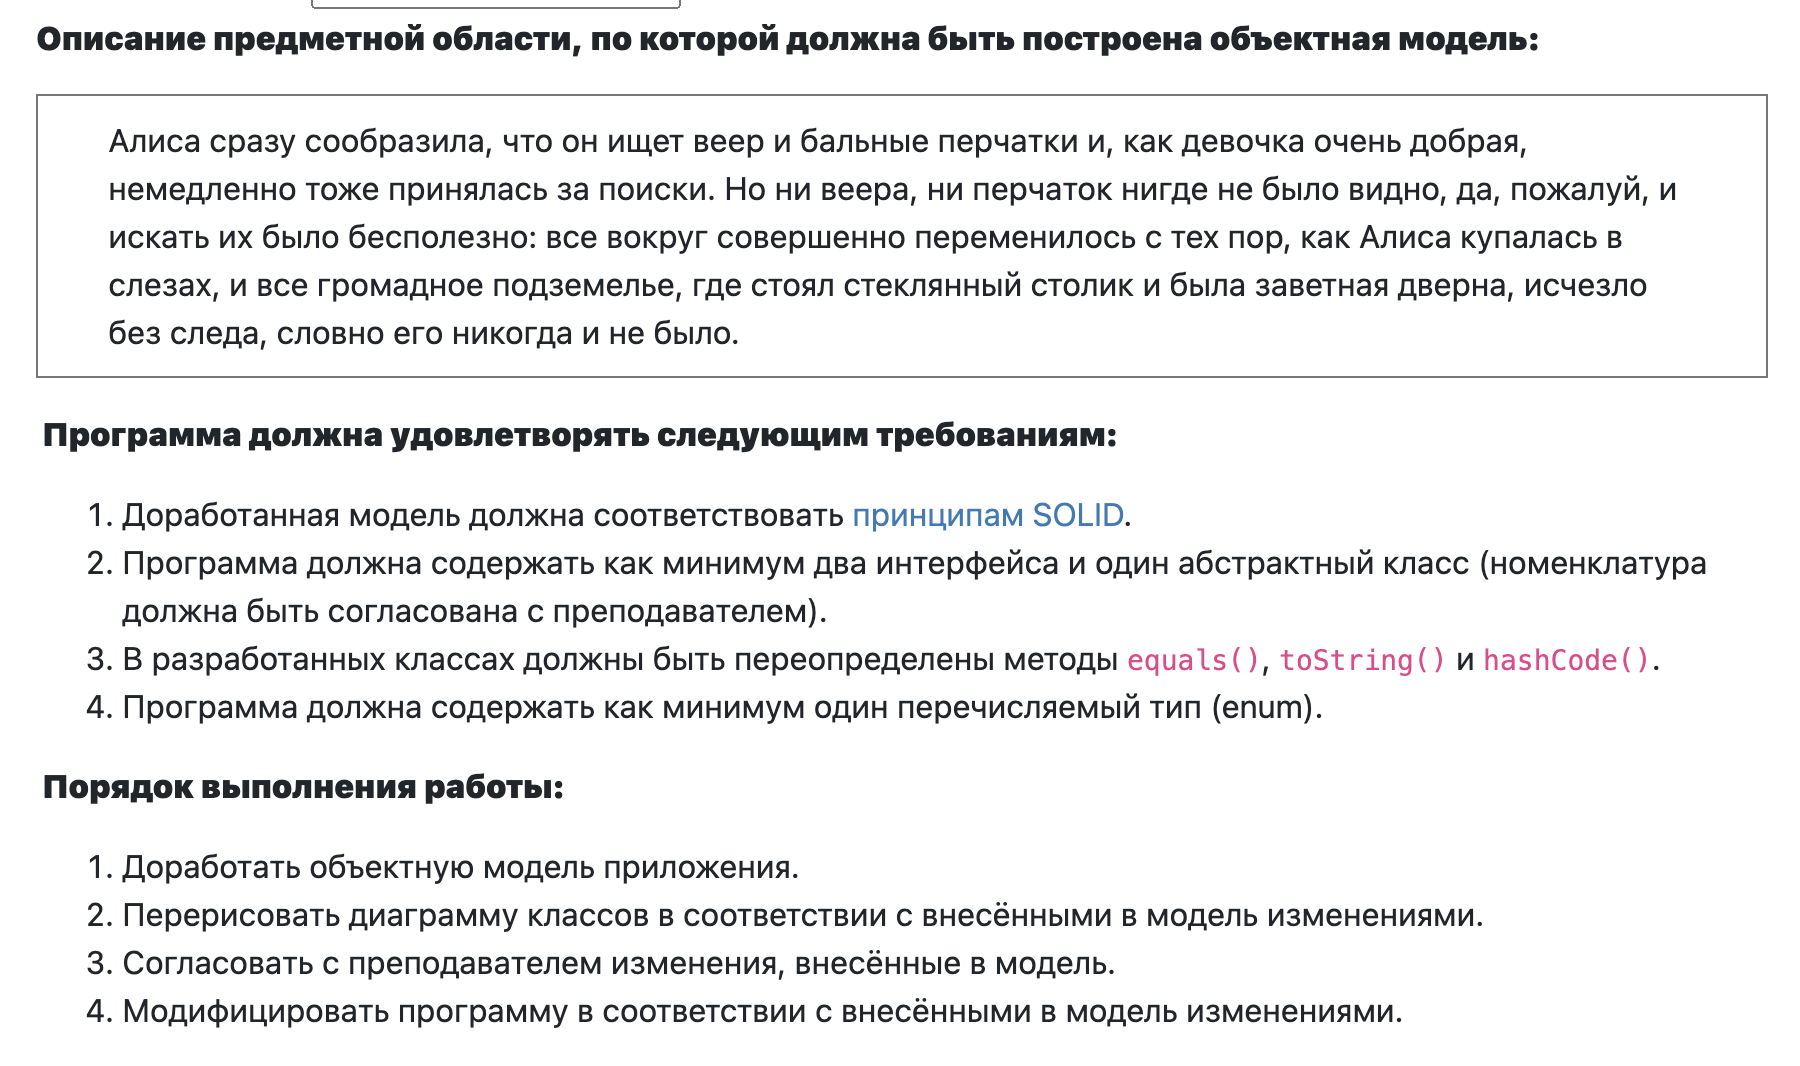
\includegraphics[width=\columnwidth]{imgs/lab3_task.png}

\section{Диаграмма классов}
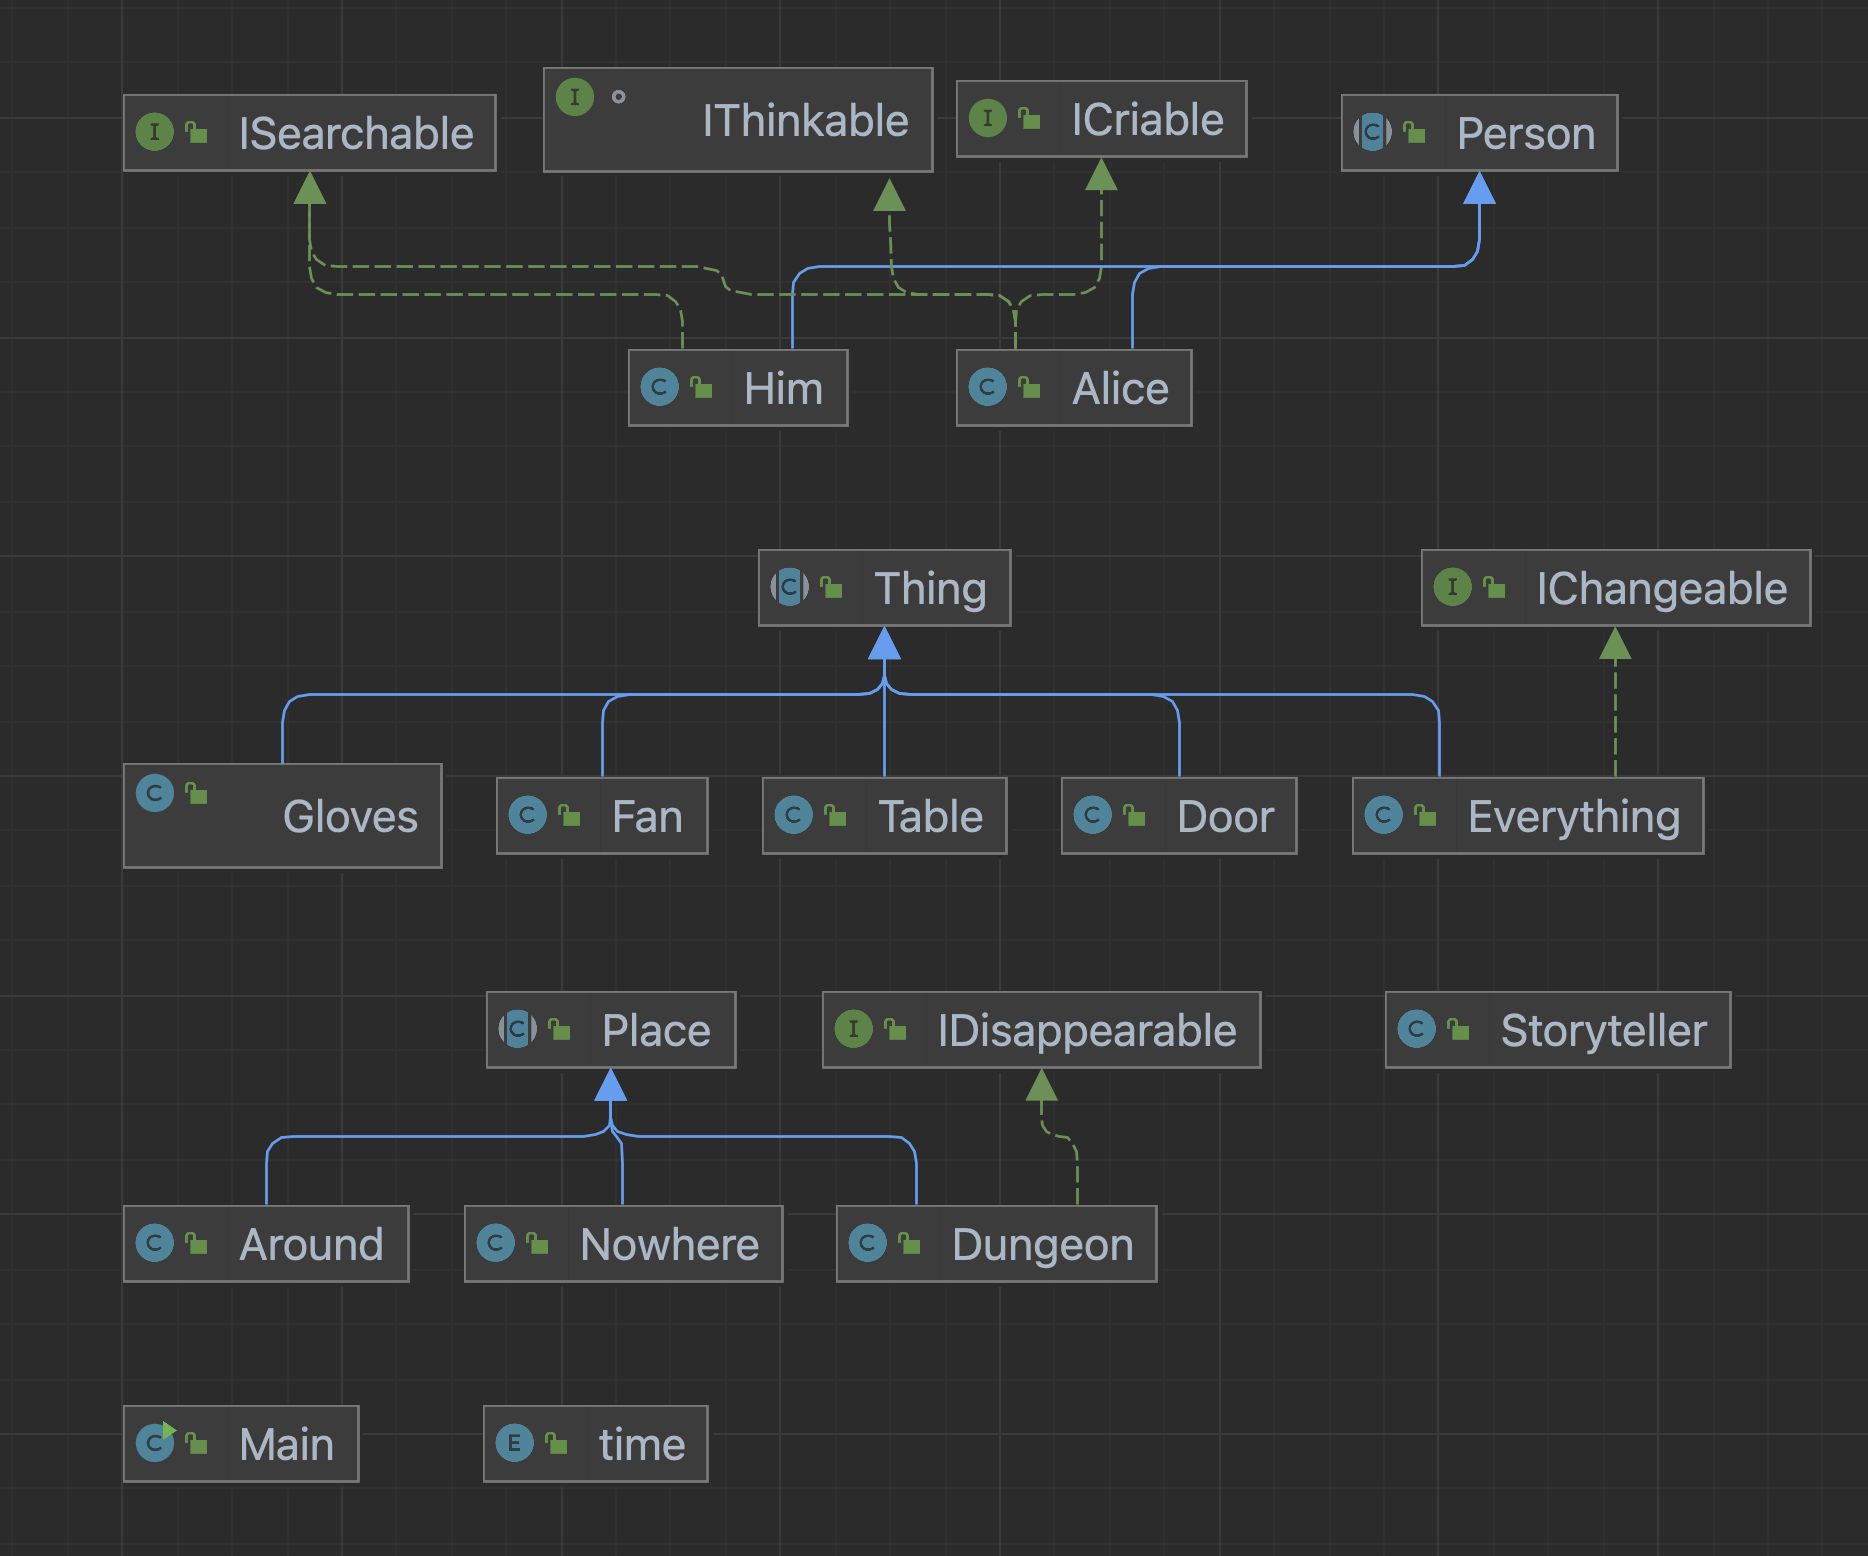
\includegraphics[width=\columnwidth]{imgs/lab3_diagram.png}

\section{Исходный код программы}
https://github.com/Ne0Ment/ITMO-proga/blob/main/lab3/src/
\begin{center}
  
\includegraphics[width=7cm]{imgs/lab3_qr.png}
\end{center}
\section{Результат выполнения}
Алиса сразу сообразила, что он ищет веер и бальные перчатки и, как девочка очень добрая, Алиса немедленно принялась за поиски. \\
Но, ни веера, ни перчаток нигде не было видно, да, пожалуй, искать их было бесполезно: все вокруг совершенно переменилось с тех пор, как Алиса купалась в слезах. \\
Громадное подземелье, где стояли стеклянный столик и заветная дверна, исчезло без следа, словно его никогда и не было. \\
\section{Вывод}
Во время выполнения лабораторной работы я узнал о принципах SOLID и STUPID а также закрепил их используя язык Java.

\end{document}